\begin{frame}{Fonts classification}\relax
    % \begin{columns}
    %     \begin{column}{0.5\textwidth}
    %          Serif
    %     \end{column}
    %     \begin{column}{0.5\textwidth}
    %          San Serif
    %     \end{column}
         
    % \end{columns}
    \begin{itemize}
        \item {\csk\scshape Serif} --- for long texts, books,..  \strut\\  
\includegraphics[width=0.9\textwidth]{fserif}
        \item {\csk\scshape Sans Serif} --- for short texts, titles, presentations,..  \strut\\  
\includegraphics[width=0.9\textwidth]{fsunserif}
        \item {\csk\scshape Typewriter} --- emulate typewriter, write code and commands   \strut\\  
\includegraphics[width=0.9\textwidth]{ftt}
        \item {\csk\scshape Other} --- Decoration etc \strut  \\  
\includegraphics[width=0.9\textwidth]{fcali}
         
    \end{itemize}
    
    \skfootnote{\vspace{-3ex}\url{https://meduza.io/feature/2017/01/29/kak-vybrat-shrift} (ru), \url{http://www.tug.dk/FontCatalogue/accanthis/} \url{http://www.tug.dk/FontCatalogue/arev/} \url{http://www.tug.dk/FontCatalogue/ascii/} \url{http://www.tug.dk/FontCatalogue/janaskrivana/}}
\end{frame}

\begin{frame}{\TeX nical classification}\relax

you have: 

\centering
standard pdf\LaTeX\ engine with ``METAFONT'' fonts:
\vspace{0.2cm}

{\footnotesize
\begin{tabular}{c|c}
\parbox{5cm}{The package has \textbf{global} usage out-of-the-box\\ you want to use it \textbf{globally}} & \parbox{5cm}{The package has \textbf{only global} usage out-of-the-box\\ you want to use it \textbf{locally}} \\\hline
\parbox{5cm}{The package has \textbf{only local} usage out-of-the-box\\ you want to use it \textbf{globally}} & \parbox{5cm}{The package has \textbf{local} usage out-of-the-box\\ you want to use it \textbf{locally}} \\
\end{tabular}}

\vspace{0.5cm}
\XeLaTeX\ with support of system-installed fonts:
\vspace{0.2cm}

{\footnotesize
\begin{tabular}{c|c}
\parbox{5cm}{The font is \textbf{global}\\ you want to use it \textbf{globally}} & \parbox{5cm}{The font is \textbf{global}\\ you want to use in \textbf{locally}} \\\hline
\parbox{5cm}{The font is \textbf{local}\\ you want to use in \textbf{globally}} & \parbox{5cm}{tThe font is \textbf{local}\\ you want to use in \textbf{locally}} \\
\end{tabular}}
\end{frame}

\begin{frame}
     \centering\Huge pdf\LaTeX
     
\end{frame}

\begin{frame}[fragile]{Global Font usage throw package with pdf\LaTeX}{where to find a font}\relax

\begin{itemize}
    \item { \url{http://www.tug.dk/FontCatalogue/allfonts.html}}
    \item { \url{https://www.ctan.org/tex-archive/fonts}}
    
\end{itemize}
\inclassFrag{Go to the first website and check some fonts!}

then just follow the instructions for the package

\end{frame}

\begin{frame}[t, fragile]{Fonts usage}{default}\relax

\samePosPicture{fnts/fontpdfdef}{9-10,25-25,30-30,34-34,38-38,42-42}\relax

\ncol\usepackage{fontenc}

\end{frame}

\begin{frame}
     \centering\huge Global Font usage throw package with pdf\LaTeX, when the package is constructed to change defaults
     
\end{frame}

%http://ctan.altspu.ru/macros/latex/doc/encguide.pdf
%https://tex.stackexchange.com/questions/25249/how-do-i-use-a-particular-font-for-a-small-section-of-text-in-my-document
\begin{frame}[t, fragile]{Fonts usage\toFrameTop{pdfLaTeX}}{Global font by loading package}\relax

\samePosPicture{fnts/fontpdfgl01}{8-10,25-25,30-30,34-34,38-38,42-42}\relax

\ncol\usepackage{<fontPackage>}\\
\Oncol\usepackage[T1]{fontenc}

     
\end{frame}

\begin{frame}[t, fragile]{Fonts usage}{Global font by loading package}\relax

\samePosPicture{fnts/fontpdfgl02}{8-10,25-25,30-30,34-34,38-38,42-42}\relax

\ncol\usepackage{<fontPackage>}\\
\Oncol\usepackage[LY1]{fontenc}
\end{frame}

\begin{frame}[t, fragile]{Fonts usage}{Global font by loading package}\relax

\samePosPicture{fnts/fontpdfgl03}{7-10,25-25,30-30,34-34,38-38,42-42}\relax

\end{frame}

\begin{frame}
     \centering\huge Local font usage throw package with pdf\LaTeX, when the package is constructed to use locally
\end{frame}

\begin{frame}[t, fragile]{Fonts usage}{Local font by loading package}\relax

\samePosPicture{fnts/fontpdflcl01}{8-10,24-25}\relax

All that is done here and bellow is just follow \url{http://www.tug.dk/FontCatalogue/allfonts.html}

\end{frame}

\begin{frame}[t, fragile]{Fonts usage}{Local font by loading package}\relax

\samePosPicture{fnts/fontpdflcl03}{7-10,24-25,29-29}\relax

There are some beautiful fonts!

\end{frame}

\inclassFrame{
\begin{frame}{Try it out!}\relax

Go to check the font \url{http://www.tug.dk/FontCatalogue/calligra/}

apply the font to the text (by example --- the following document)

\lstinputlisting{fnts/fontpdfTASK.tex}

after you succeeded --- add \ccol\bfseries\ to make the font bold
     
\end{frame}
}

\begin{frame}[t, fragile]{Fonts usage}{Local font by loading package}\relax

\samePosPicture{fnts/fontpdflcl02}{8-10,24-25, 31-31, 36-36}\relax

\end{frame}


\begin{frame}[fragile]{Fonts usage\premagicPage}{Understanding warning}\relax

Last example provides warning:\\ 
{\csk \verb|LaTeX Font Warning: Font shape `T1/calligra/bx/n' undefined|}

Sometimes you can find something like {\csk\verb|OT1/cmr/m/n/10|}

How to read it?
\strut
\incPause

\centering 
\begin{tabular}{c|c|c|c|c}
T1&calligra&bx&n&\\ 
OT1&cmr&m&it&10\\\hline
\large encoding & font family & series & shape & font size
\end{tabular}
\skfootnote{\normalfont \url{http://mirrors.ctan.org/macros/latex/doc/fntguide.pdf}: 2.1, \normalfont\url{http://mirrors.ctan.org/macros/latex/doc/encguide.pdf}}
\end{frame}

\begin{frame}[fragile]{Fonts usage\magicPage}{Understanding warning}\relax

\begin{columns}[t]
\begin{column}{0.5\textwidth}

Most common encodings\strut\hrule

\begin{tabular}{rl}
     OT1 & TEX text\\
     T1 & TEX extended text\\
     OML & TEX math italic\\
     OMS & TEX math symbols\\ 
     OMX & TEX math large symbols\\
     U & Unknown\\ 
     L<xx>& local encoding
\end{tabular}
\end{column}

\begin{column}{0.5\textwidth}

Some common families\strut\hrule

\begin{tabular}{r>{\footnotesize}l}

     cmr & Computer Modern Roman\\ 
     cmss & Computer Modern Sans\\ 
     cmtt & Computer Modern Typewriter\\ 
     cmm & Computer Modern Math Italic\\ 
     cmsy & Computer Modern Math Symbols\\ 
     cmex &  Computer Modern Math Extensions\\ 
     ptm & Adobe Times\\ 
     phv & Adobe Helvetica\\ 
     pcr &Adobe Courier
\end{tabular}
\end{column}
     
\end{columns}
\cprotect\skfootnote{more families: \overC{https://www.overleaf.com/learn/latex/Font_typefaces} \normalfont \url{http://mirrors.ctan.org/macros/latex/doc/fntguide.pdf}: 2.1\\
Look at the source code to understand how the right table was created (\verb|>{\footnotesize}| and \verb|\usepackage{array}|)
}
\end{frame}

\begin{frame}[fragile]{Fonts usage\magicPage}{Understanding warning}\relax
\centering
\begin{columns}[t]
\begin{column}{0.5\textwidth}
\centering

Most common values for series\strut\hrule

\begin{tabular}{rl}
     t & thin\\
     m &Medium\\ 
     b &Bold \\
     bx & Bold extended\\ 
     sb &Semi-bold\\ 
     c & Condensed
\end{tabular}
\end{column}

\begin{column}{0.5\textwidth}

Most common values for shape\strut\hrule

\begin{tabular}{rl}
n & Normal \scriptsize(that is 'upright' or 'roman') \\ 
it & Italic\\  
sl & Slanted \scriptsize(or 'oblique') \\ 
sc &Caps and small caps
\end{tabular}
\end{column}
     
\end{columns}
\cprotect\skfootnote{ \normalfont \url{http://mirrors.ctan.org/macros/latex/doc/fntguide.pdf}: 2.1
}
\end{frame}

\begin{frame}
\magicPage
     \centering\huge Global font usage throw package with pdf\LaTeX, when the package is constructed to use locally
     
\end{frame}

\begin{frame}[fragile]{Algorithm\magicPage}\relax

You need to figuraute the {\csk Font Family}
\begin{enumerate}
     \item Check the package documentation
     \item (Remember, that not all fonts provide all series and shapes!)
     \item If manual is unreachable, get the Family directly: \ccol{\showthe}\ccol{\font} and see {\csk logs}:
\end{enumerate}

\logshow{fnts/fontpdfNONDEFgl01}{8-10, 19-21}{1-4}

\begin{enumerate}
    \setcounter{enumi}{3}
    \item get the family ({\csk hmin}) and use it! (next slide)
     
\end{enumerate}
\skfootnote{\stExC{https://tex.stackexchange.com/questions/25249/how-do-i-use-a-particular-font-for-a-small-section-of-text-in-my-document/25251\#25251}}     
\end{frame}

\begin{frame}[t, fragile]{Fonts usage\magicPage}{global}\relax

\samePosPicture{fnts/fontpdfNONDEFgl01}{8-10,15-15,23-23,27-27,31-31}\relax

\verb|\renewcommand{|\ccol{\rmdefault}\verb|}<family_name>|

\skfootnote{\stExC{https://tex.stackexchange.com/questions/25249/how-do-i-use-a-particular-font-for-a-small-section-of-text-in-my-document/25251\#25251} \normalfont \url{http://mirrors.ctan.org/macros/latex/doc/fntguide.pdf}: 2.4}
\end{frame}

\begin{frame}
\magicPage
     \centering\huge Local font usage throw package with pdf\LaTeX, when the package is constructed to change defaults
     
\end{frame}

\begin{frame}[fragile]{Algorithm\magicPage}\relax

You need to figuraute the {\csk Font Family}
\begin{enumerate}
     \item Check the package documentation
     \item If manual is unreachable, get the Family directly:
     \ccol{\rmdefault} or \ccol{\familydefault}
\end{enumerate}

\samePosPicture{fnts/fontpdfNONDEFlcl01}{8-10, 17-18}

\begin{enumerate}
    \setcounter{enumi}{2}
    \item remember the family ({\csk ybd2j}) to use it (next slide)
     
\end{enumerate}

\end{frame}

\begin{frame}[fragile]{Algorithm\magicPage}\relax

\samePosPicture{fnts/fontpdfNONDEFlcl02}{8-10, 15-16, 22-23}

\begin{enumerate}
    \setcounter{enumi}{3}
    \item Change the encoding and font family to defaults (\verb|\renewcommand{|\ccol\encodingdefault\verb|}{|\ccol{OT1}\verb|}|, \verb|\renewcommand{|\ccol\rmdefault\verb|}{|\ccol{cmr}\verb|}|)
     
\end{enumerate}
\skfootnote{\stExC{https://tex.stackexchange.com/questions/25249/how-do-i-use-a-particular-font-for-a-small-section-of-text-in-my-document/25251\#25251} \normalfont \url{http://mirrors.ctan.org/macros/latex/doc/fntguide.pdf}: 2.2}
\end{frame}

\begin{frame}[t, fragile]{Fonts usage\magicPage}{locally}\relax
How to change font:
\begin{itemize}
    \item \ccol\fontencoding\ will change the encoding
    \item \ccol\fontfamily\ will change family
    \item \ccol\fontseries\ wil change series 
    \item \ccol\fontshape\ will change shape 
    \item \ccol\fontsize\ will change font size 
\end{itemize}
... and {\large \ccol\selectfont}\ after font change!

\inclassFrag{why do we need the ending-command like \ccol\selectfont ?}
We need \ccol{\selectfont} because while changing the font we can be in an inconsistent state: for example, we change the encoding, but now there is no such family as an old one!

\skfootnote{\stExC{https://tex.stackexchange.com/questions/25249/how-do-i-use-a-particular-font-for-a-small-section-of-text-in-my-document/25251\#25251} \normalfont \url{http://mirrors.ctan.org/macros/latex/doc/fntguide.pdf}: 2.2}
\end{frame}

\begin{frame}
     \centering\Huge \XeLaTeX\ and Lua\TeX
     
\end{frame}

\begin{frame}{Fonts usage}{XeLaTeX and LuaTeX}\relax
     \begin{enumerate}
         \item You can use practically all fonts from pdf\LaTeX
         \item You can use OpenType (OTF), TrueType (TTF) fonts. They usually install in your system.
          
     \end{enumerate}
\end{frame}

\begin{frame}
     \centering\huge Global font usage throw global-available font with \XeLaTeX
     
\end{frame}

\begin{frame}[fragile]{Font usage}{default}\relax

\samePosPicture{fnts/fontXedef}{9-9,24-24,29-29,33-33,37-37,41-41}

\verb|\usepackage{|\ccol{fontspec}\verb|}|
\end{frame}

\begin{frame}[fragile]{Font usage}{global}\relax

\samePosPicture{fnts/fontXegl01}{7-8,24-24,29-29,33-33,37-37,41-41}

\ccol\setmainfont<font-name>
\skfootnote{\wikiC{https://en.wikibooks.org/wiki/LaTeX/Fonts\#Using_TTF_and_OTF_fonts} \overC{https://www.overleaf.com/learn/latex/XeLaTeX} \stExC{https://tex.stackexchange.com/questions/25249/how-do-i-use-a-particular-font-for-a-small-section-of-text-in-my-document/37251\#37251}}
\end{frame}

\begin{frame}[fragile]{Font usage\premagicPage}{global}\relax

\samePosPicture{fnts/fontXegl02}{7-8,24-24,29-29,33-33,37-37,41-41}
\ccol\setmainfont<font-name>

\skfootnote{\wikiC{https://en.wikibooks.org/wiki/LaTeX/Fonts\#Using_TTF_and_OTF_fonts} \overC{https://www.overleaf.com/learn/latex/XeLaTeX} \stExC{https://tex.stackexchange.com/questions/25249/how-do-i-use-a-particular-font-for-a-small-section-of-text-in-my-document/37251\#37251}}
\end{frame}


\begin{frame}[fragile]{Font usage\magicPage}{global}\relax
\begin{itemize}
    \item \ccol\setmainfont\ sets the roman font
    \item \ccol\setsansfont\ sets the sans font
    \item \ccol\setmonofont\ sets the monospace font 
     
\end{itemize}

\skfootnote{\wikiC{https://en.wikibooks.org/wiki/LaTeX/Fonts\#Using_TTF_and_OTF_fonts} \overC{https://www.overleaf.com/learn/latex/XeLaTeX} \stExC{https://tex.stackexchange.com/questions/25249/how-do-i-use-a-particular-font-for-a-small-section-of-text-in-my-document/37251\#37251}}
\end{frame}

\begin{frame}
     \centering\huge Local font usage throw global-avaliable font with \XeLaTeX
\end{frame}

\begin{frame}[fragile]{Font usage\magicPage}{local}\relax

\samePosPicture{fnts/fontXelcl01}{8-8,23-24,33-34}
\ccol\fontspec<font-name>

\skfootnote{\stExC{https://tex.stackexchange.com/questions/25249/how-do-i-use-a-particular-font-for-a-small-section-of-text-in-my-document/37251\#37251}}
\end{frame}

\begin{frame}[fragile]{Font usag\magicPagee}{local}\relax

\samePosPicture{fnts/fontXelcl02}{8-8,18-18,23-24,33-34}
\ccol\newfontfamily\ --- more effective way

\skfootnote{\stExC{https://tex.stackexchange.com/questions/25249/how-do-i-use-a-particular-font-for-a-small-section-of-text-in-my-document/37251\#37251}}
\end{frame}

\begin{frame}
     \centering\huge Global font usage throw local-avaliable font with \XeLaTeX
\end{frame}
\begin{frame}[fragile]{Font usage}{global}\relax

\samePosPicture{fnts/fontXeNNgl01}{7-8,24-24,29-29,33-33,37-37,41-41}
\ccol\setmainfont<font-filename>

\skfootnote{\overC{https://www.overleaf.com/learn/latex/XeLaTeX} \\
from \url{https://www.fontsquirrel.com/fonts/lato}}
\end{frame}

\begin{frame}[fragile]{fontspec's commands optional params\magicPage}\relax
\begin{itemize}
    \item BoldFont = ⟨font name⟩
\item ItalicFont = ⟨font name⟩
\item BoldItalicFont = ⟨font name⟩
\item SlantedFont = ⟨font name⟩
\item BoldSlantedFont = ⟨font name⟩
\item SmallCapsFont = ⟨font name⟩
\item UprightFont = ⟨font name⟩
\end{itemize}
     
     \skfootnote{\url{http://mirrors.ctan.org/macros/latex/contrib/fontspec/fontspec.pdf}: 3.1}
\end{frame}

\begin{frame}\magicPage
     \centering\huge Local font usage throw local-avaliable font with \XeLaTeX
\end{frame}

\begin{frame}[fragile]{Font usage\magicPage}{local}\relax

\samePosPicture{fnts/fontXeNNlcl01}{8-8,23-24,33-34}
\ccol\fontspec<font-name>

\end{frame}

\begin{frame}[fragile]{Font usage\magicPage}{local}\relax

\samePosPicture{fnts/fontXeNNlcl02}{8-8,18-18,23-24,33-34}
\ccol\newfontfamily\ --- more effective way


\end{frame}

\begin{frame}{How to find a font}\relax
\centering
     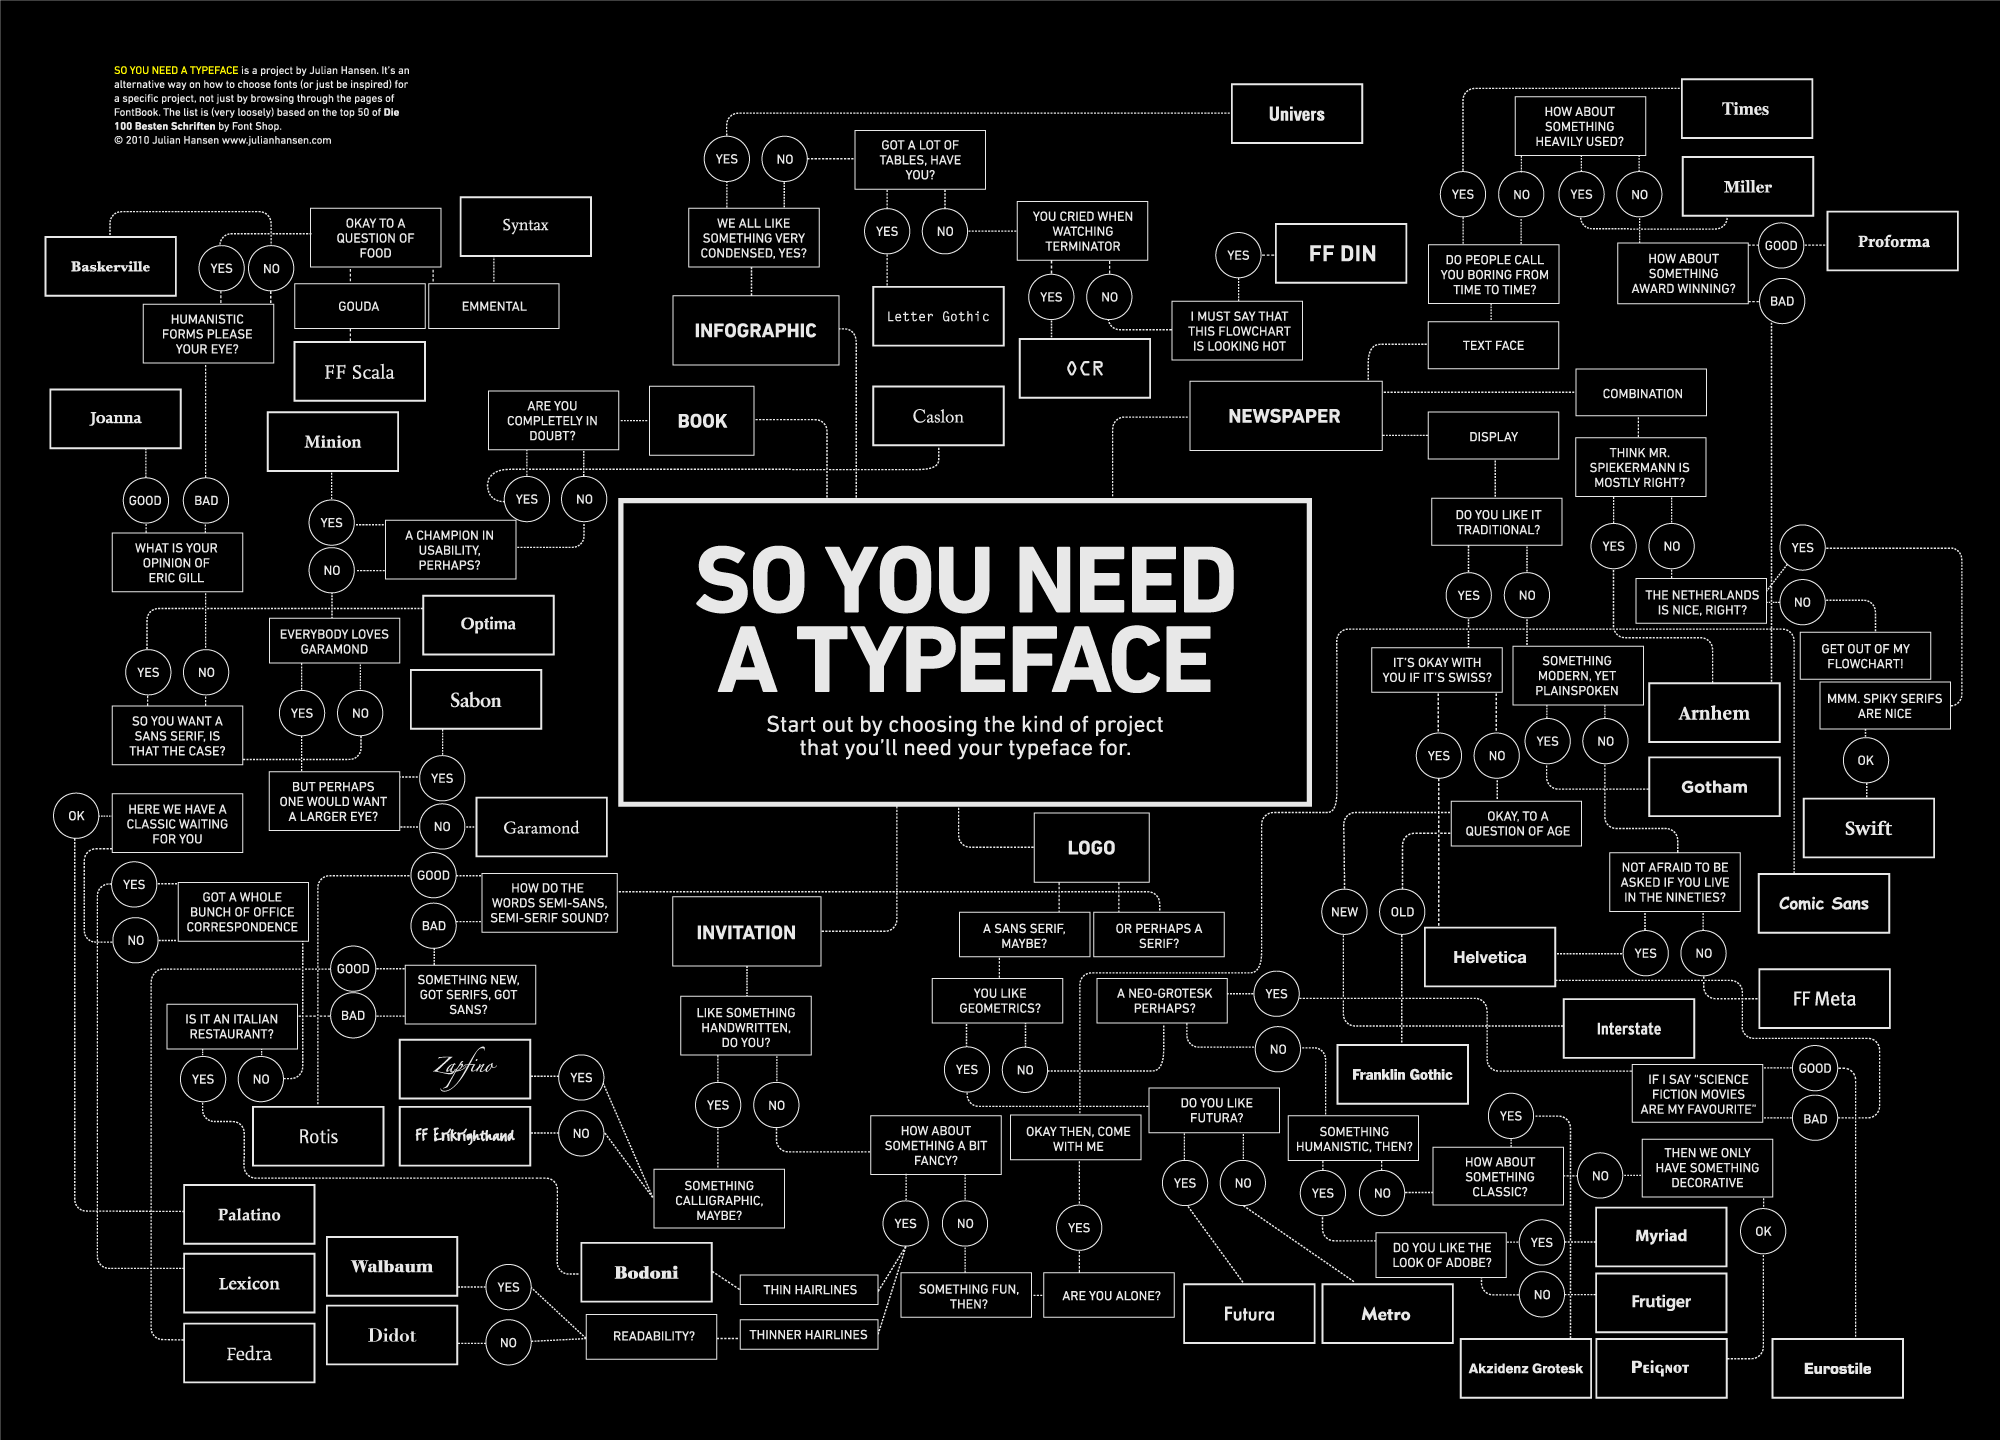
\includegraphics[height=0.8\textheight]{choosing-fonts}
     
     \skfootnote{\url{https://www.labnol.org/home/choose-fonts-with-flowchart/13488/}}
\end{frame}

\begin{frame}{Useful links}\relax
\begin{itemize}
    \item {\csk \url{http://www.tug.dk/FontCatalogue/}} avaliable at \LaTeX\ fonts 
    \item {\csk \url{https://www.fontsquirrel.com/}} font catalogue 
    \item {\csk \url{https://www.fontsquirrel.com/matcherator}} identify font by picture
    \item {\csk \url{https://www.fonts-online.ru/fonts/russian}} fonts with cyrillic 
    \item {\csk \url{http://allfont.ru/free/}} fonts with cyrillic 
    \item {\csk \url{https://fonts.google.com/?subset=cyrillic}} fonts with cyrillic
    \item {\csk \url{https://wordmark.it/}} quick look of how your text will look like
     
\end{itemize}
\end{frame}

\begin{frame}{Useful tips: Font pairs}\relax
    Don't use too many fonts in your document! The best choice is two-three different fonts.
    
    How to choose font pairs? 
    
    \begin{itemize}
        \item \url{https://www.fastprint.co.uk/blog/the-art-of-mixing-typefaces.html} cheat list
        \item \url{https://www.canva.com/font-combinations/} combinator
        \item \url{https://fontpair.co/} list 
        \item \url{http://font-combinator.com/} combinator
        \item \url{http://www.joustmultimedia.com/blog/post/the-art-of-combining-fonts} some tips
         
    \end{itemize}
     \skfootnote{from \url{https://freelance.today/poleznoe/15-servisov-dlya-podbora-shriftovyh-par.html}}
\end{frame}

